
%\documentclass[a4paper,twocolumn,psfig,subfigure,epsfig,fleqn,ausarbeitung,amssmb,float,caption,fontenc]{article}
\documentclass[a4paper,psfig,subfigure,epsfig,ausarbeitung,amssmb,float,caption,fontenc]{article}
 
\pagestyle{empty}

\bibliographystyle{plain}

\usepackage{hyperref}
\usepackage{enumitem}
\usepackage{subcaption}
\usepackage{graphicx}
\usepackage[section]{placeins} % to avoid figures floating out of the current section
\usepackage{amsmath}
\usepackage{amsfonts}

%set dimensions of columns, gap between columns, and paragraph indent

\setlength{\textheight}{24.7 cm}
\setlength{\columnsep}{1 cm}
\setlength{\textwidth}{16 cm}
%\setlength{\footheight}{0.0 cm}
\setlength{\topmargin}{0.0 cm}
\setlength{\headheight}{0.0 cm}
\setlength{\headsep}{-0.3 cm}
\setlength{\oddsidemargin}{0.0 cm}
\setlength{\parindent}{0.7 cm}
%\setlength{\mathindent}{20mm}

% set page counter if document is part of proceedings
\setcounter{page}{23}
\renewcommand{\floatpagefraction}{0.9}
\renewcommand{\textfraction}{0.1}
\DeclareMathOperator*{\argmin}{arg\,min}

%\renewcommand{\captionlabelfont}{\fontfamily{phv}\fontseries{bx}\fontsize{10}{10pt}\selectfont}
%\renewcommand{\captionfont}{\fontfamily{phv}\fontsize{10}{12pt}\selectfont}
%\setlength{\captionmargin}{0.5 cm}

\makeatletter
\makeatother
\def\RR{\hbox{I\kern-.2em\hbox{R}}}


\begin{document}

%don't want date printed
\date{}

%make title bold and 14 pt font (Latex default is non-bold, 16pt) 
\title{%~\\
%  ~\\
  \fontsize{14}{14pt} \bf Computer Vision Exercise II: Report}

\author{~\\
  ~\\
  \fontsize{12}{12pt}
  \begin{tabular}[t]{c c c}
  {\bf Alexander Cech}                    & {\bf Hamed Jafari-Sahamieh}             & {\bf Patrick Link}                      \\
  \small{Student of Visual Computing}     & \small{Student of Visual Computing}     & \small{Student of Visual Computing}     \\
  \small{Vienna University of Technology} & \small{Vienna University of Technology} & \small{Vienna University of Technology} \\
  \small{e08900070@student.tuwien.ac.at}  & \small{e09826767@student.tuwien.ac.at}  & \small{e11728332@student.tuwien.ac.at}  \\
  \end{tabular}
  ~\\ 
%  ~\\ ~\\
  \normalsize
%  {\bf ABSTRACT} \\ 
%  \noindent
%  \hspace{0.2cm}
%  \begin{minipage}[c]{15cm}
%  \normalsize This is my abstract.  This is my abstract.  This is my
%    abstract.  This is my abstract.  This is my abstract.  This is my
%    abstract.  This is my abstract.  This is my abstract.  This is my
%    abstract.  This is my abstract.  This is my abstract.  This is my
%    abstract.\\
%  \end{minipage}
%  ~\\ ~\\ ~\\
  \normalsize
%  {\bf KEYWORDS} \\ 
%  \normalsize
%  Keyword1, Keyword2, Keyword3, Keyword4, Keyword5, Keyword6.
  }

\maketitle

%I don't know why I have to reset thispagestyle, but otherwise get page numbers 
\normalfont
\thispagestyle{empty}

%\section{Introduction}
%\label{sec:introduction}
%
%


\section{Assignment 4: Image Stitching}
\label{sec:assignment4}


\subsection{SIFT Interest Point Detection}

In the first step we use the SIFT algorithm for key point detection. As we do not need the key descriptors at this stage, we only acquire the position of each key point along with their scale and orientation. SIFT uses the Difference of Gaussians (DoG) to approximate LoG. To define different scales, the SIFT algorithm creates a minimum of five different Gaussian images per octave, the difference of these images (DoGs) are then used for Maxima detection, similar to blob detection algorithm. 

\begin{figure}[h]
	\centering
	\begin{tabular}{cc}
	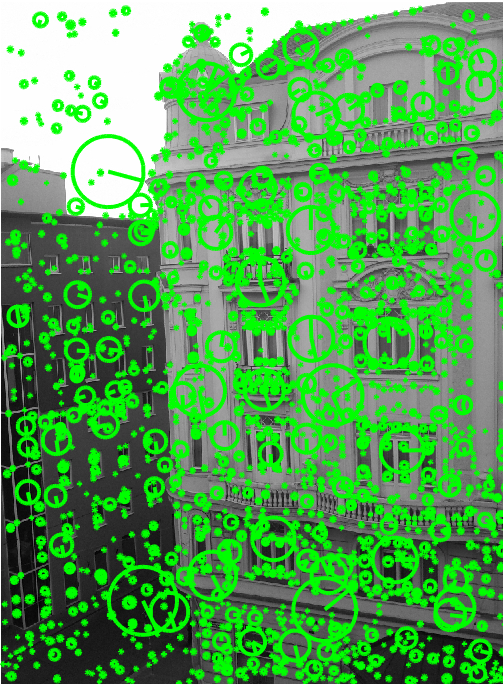
\includegraphics[width=0.48\textwidth]{figures/vl_plotframe_officeview1.png} &
	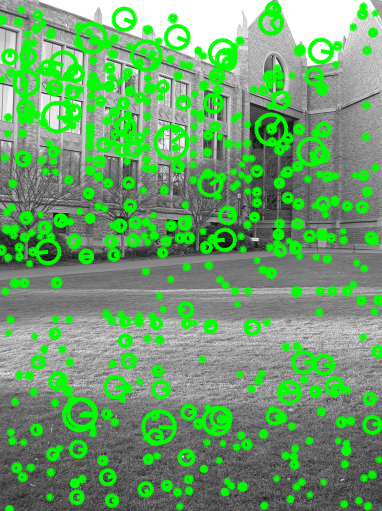
\includegraphics[width=0.48\textwidth]{figures/vl_plotframe_campus4.png} 

	\end{tabular}
	\caption{SIFT key point detection: scale and orientation of key points.}
	\label{fig:a4:vlplotframe}
\end{figure}

To find the orientation of the key points, depending on the scale, a region around the key point center is chosen. The magnitudes and orientations are calculated for each pixel in this region, and the result is placed in a histogram made of 36 bins (10degrees per bin). The highest point of the histogram is the orientation of the key point. Any other peak close to the highest point is converted into a new key point (same position and scale, but with a different orientation). The key point orientation is important, because further calculations (descriptors) will be relative to this orientation, which ensures orientation invariance for matching key points.

The function \texttt{vl\_plotframe} illustrates the results. The circle corresponds to the associated scale of the key point and the line is its orientation as visualized in Figure \ref{fig:a4:vlplotframe}.

\subsection{Interest Point Matching and Image Registration}

Similar to step A, first we extract all key points via SIFT, this time along with the associated descriptors of each key point. The descriptors are an array of 128 numbers constructed as follows: First the 16x16 window around the key point is broken down into smaller 4x4 windows. Within each of the 16 windows the gradients are calculated and subsequently put into an 8 bin histogram (45 degrees each). The magnitude added by each gradient also depends on the distance from the key point (using gaussian weights). 

Each of the 128 resulting numbers will be normalized and reduced by the key point's orientation (to ensure orientation invariance) and subsequently clamped at 0.2 (to ensure illumination invariance) before being normalized to unit vector again.

\begin{figure}[h]
	\centering
	\begin{tabular}{cc}
	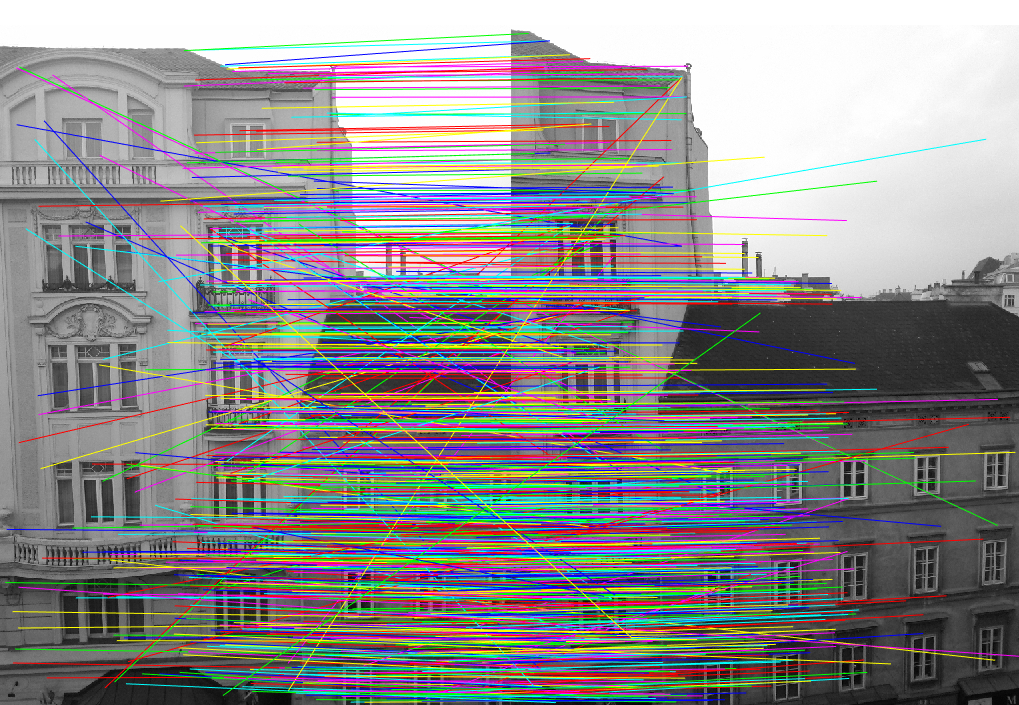
\includegraphics[width=0.75\textwidth]{figures/vl_ubcmatch1.png} \\
	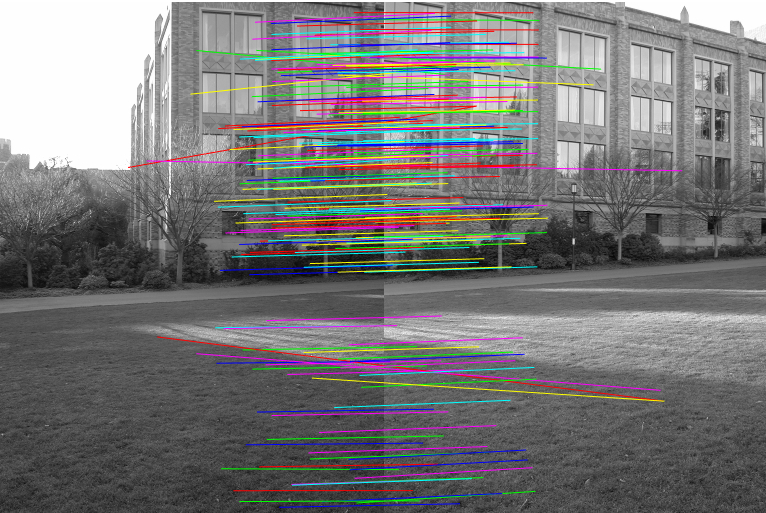
\includegraphics[width=0.75\textwidth]{figures/vl_ubcmatch2.png} 

	\end{tabular}
	\caption{The resuts of \texttt{vl\_ubcmatch}. }
	\label{fig:a4:ubcmatch}
\end{figure}

\texttt{vl\_ubcmatch} is used as a first, basic, matching step. For each descriptor in the first image, \texttt{vl\_ubcmatch} attempts to find the closest descriptor in the target image using L2 norm of the difference between the two. This basic algorithm may consequently return many false positive matches as well. The result is illustrated by Figure \ref{fig:a4:ubcmatch}.

To eliminate potential false positive matches, a RANSAC scheme is applied. Basically, we estimate the correct homography  by using 4 random sample matches out of all matches found by \texttt{vl\_ubcmatch} before applying them to all other key points via \texttt{transformPointsforward}. Subsequently we keep only those matches which are inliers, that is their euclidean distance is smaller than a certain threshold T. The RANSAC algorithm is applied N times and the homography  with the largest number of inliers is returned as the correct estimation. 

The result is presented in Figure \ref{fig:a4:ransac}.

\begin{figure}[h]
	\centering
	\begin{tabular}{cc}
	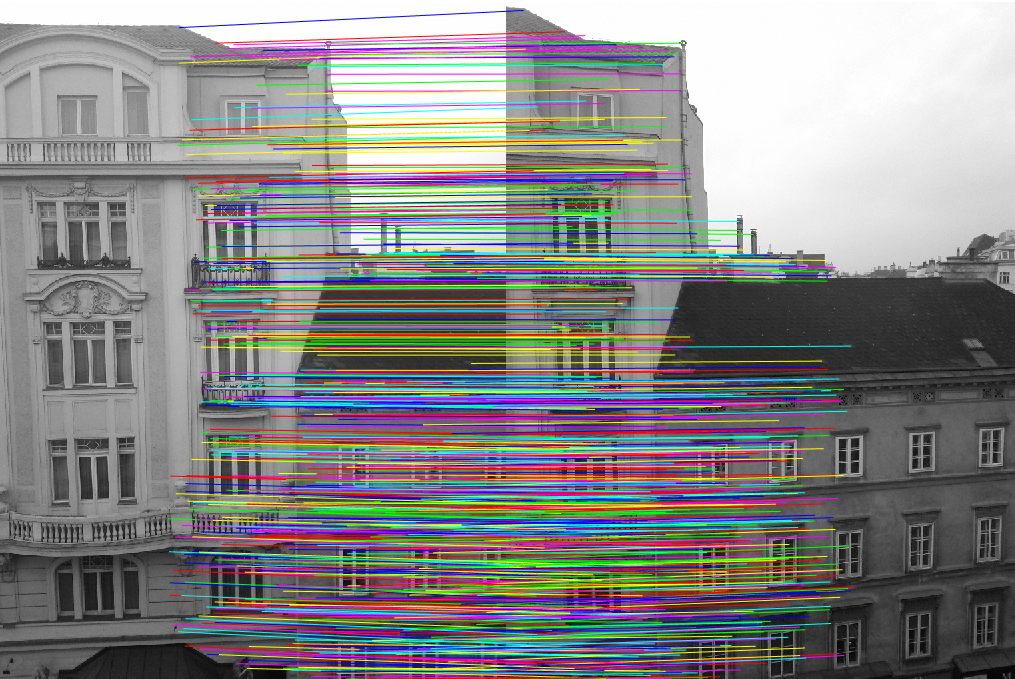
\includegraphics[width=0.8\textwidth]{figures/ransac1.png} \\
	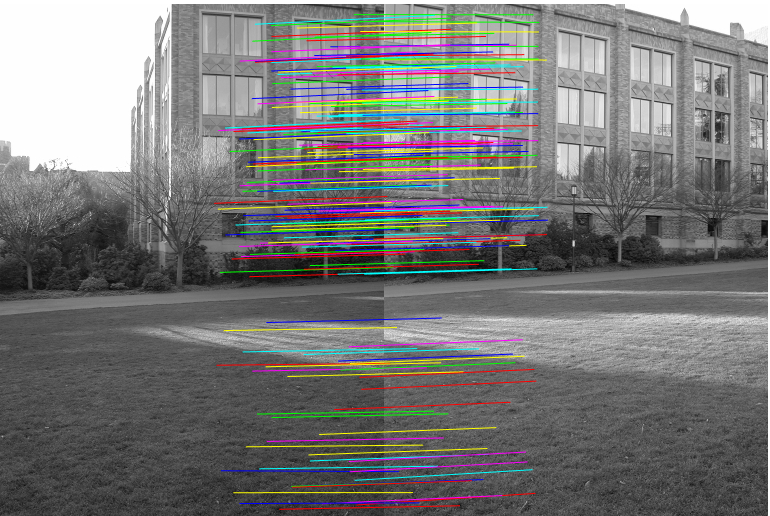
\includegraphics[width=0.8\textwidth]{figures/ransac2.png} 

	\end{tabular}
	\caption{The matched key points after applying RANSAC. }
	\label{fig:a4:ransac}
\end{figure}


Figure \ref{fig:a4:ransac_removes} illustrates the potential false positive matches that are eliminated after applying RANSAC.


\begin{figure}[h]
	\centering
	\begin{tabular}{cc}
	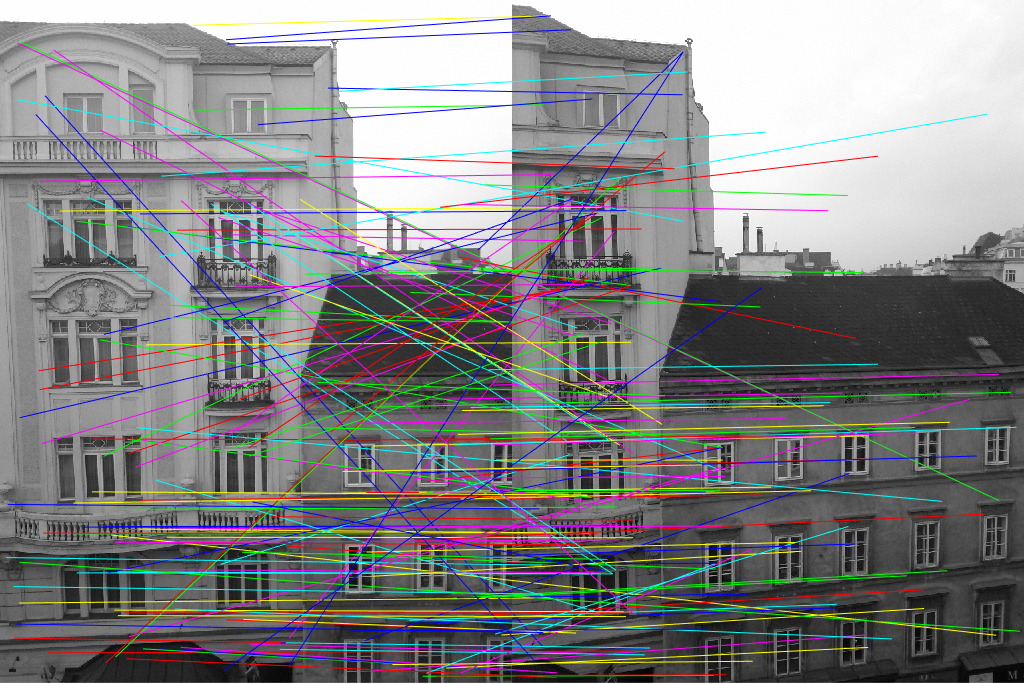
\includegraphics[width=0.45\textwidth]{figures/ransac_removes1.png} &
	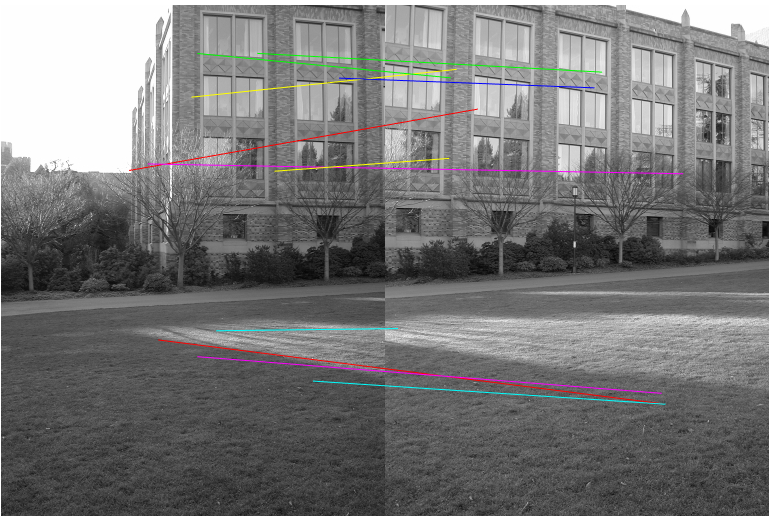
\includegraphics[width=0.45\textwidth]{figures/ransac_removes2.png} 

	\end{tabular}
	\caption{Potentially false positive matches estimated by \texttt{vl\_ubcmatch}. }
	\label{fig:a4:ransac_removes}
\end{figure}


\begin{figure}[h]
	\centering
	\begin{tabular}{cc}
	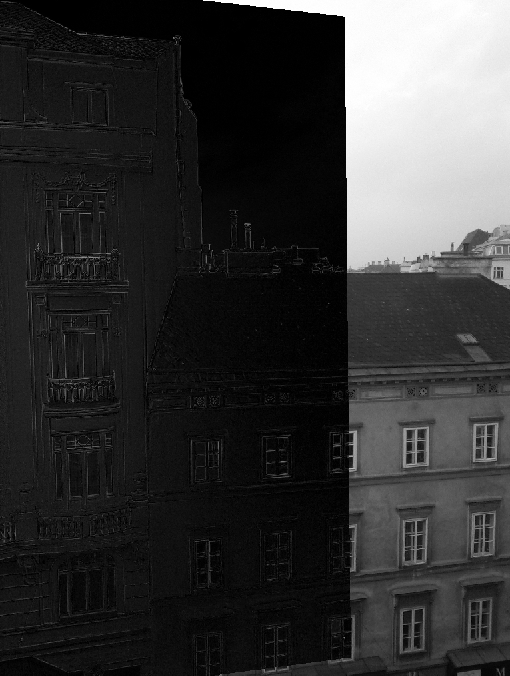
\includegraphics[width=0.23\textwidth]{figures/diff1.png} 
	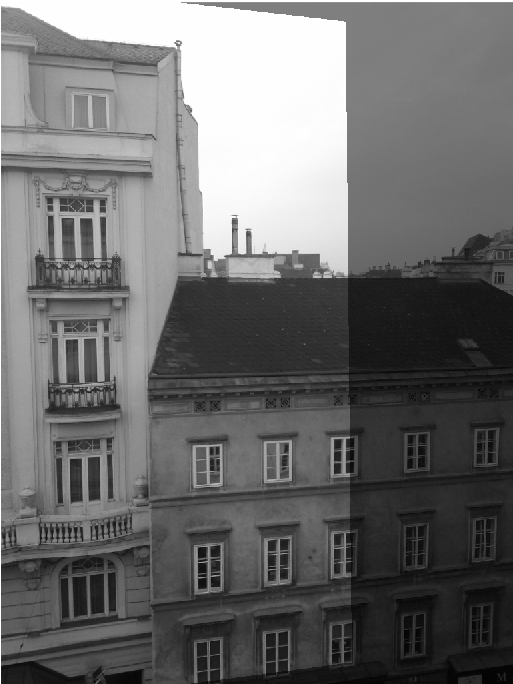
\includegraphics[width=0.23\textwidth]{figures/overlay1.png} 
	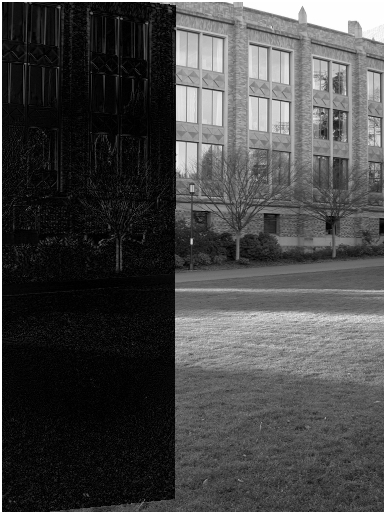
\includegraphics[width=0.23\textwidth]{figures/diff2.png} 
	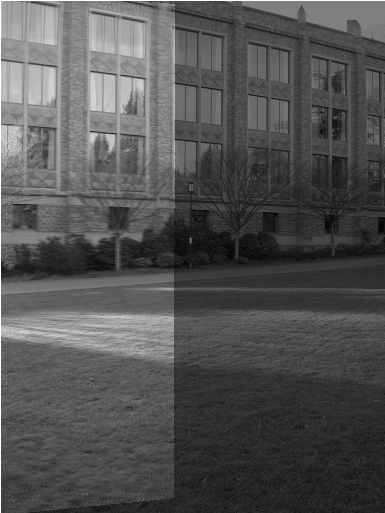
\includegraphics[width=0.23\textwidth]{figures/overlay2.png} 

	\end{tabular}
	\caption{Difference and overlay view of aligned images.}
	\label{fig:a4:diffs}
\end{figure}


After applying the above steps the images are already well aligned as presumed. Figure \ref{fig:a4:diffs} shows a collection of absolute differences of pairs of matched images. 



\begin{figure}[h]
	\centering
	\begin{tabular}{cc}
	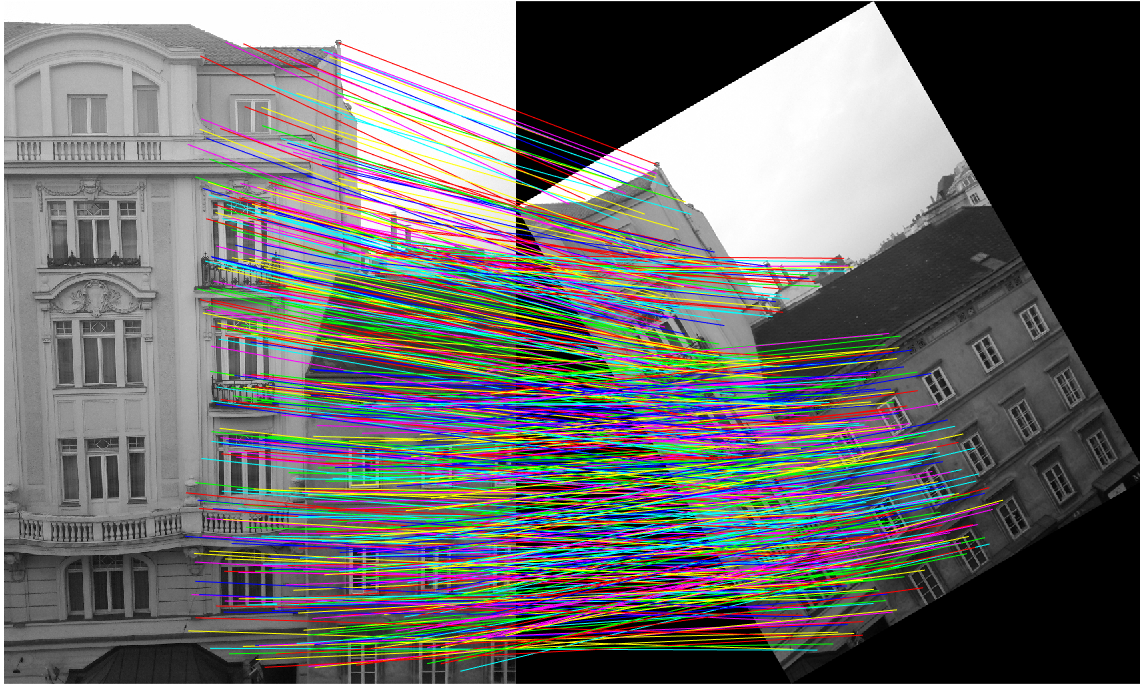
\includegraphics[width=0.59\textwidth]{figures/rotation_ransac.png} &
	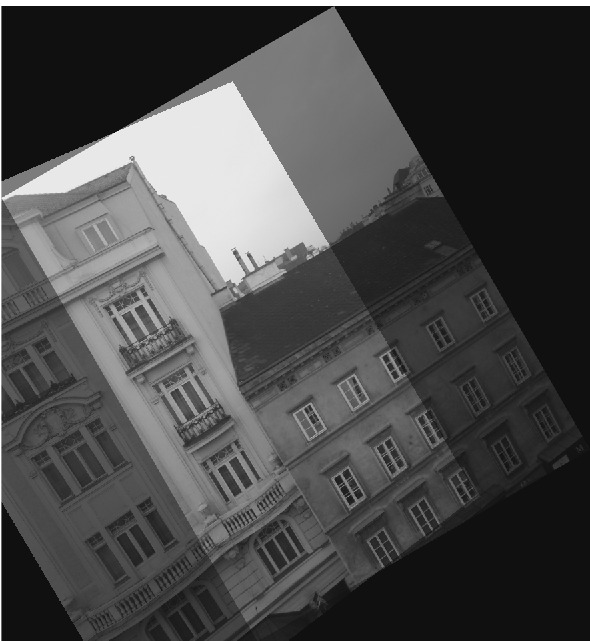
\includegraphics[width=0.33\textwidth]{figures/rotation_overlay.png} 

	\end{tabular}
	\caption{Post RANSAC matches after rotating and rescaling and the aligned result.}
	\label{fig:a4:rotationscale}
\end{figure}

\FloatBarrier % keep figures above!

As described above, the gradient orientation of each pixel is reduced by the key point orientation before being added to the associated histogram. Therefor the result should be invariant to changes in image rotation. Additionally the SIFT algorithm is also scale invariant as described in the first section. This can be seen as illustrated by Figure \ref{fig:a4:rotationscale}.

\subsection{Image Stitching}

To stitch images together for the purpose of creating a panorama view, first the homography is estimated between each pair of adjacent images. An image is selected as reference image (one in the middle of panorama) and utilizing the homographies estimated before, the homography of each image to the reference image is also estimated. Finally each image can be projected into its correct place within the panorama. The results can be viewed on figures \ref{fig:a4:pano1} and \ref{fig:a4:pano2}.

\begin{figure}[h]
	\centering
	\begin{tabular}{cc}
	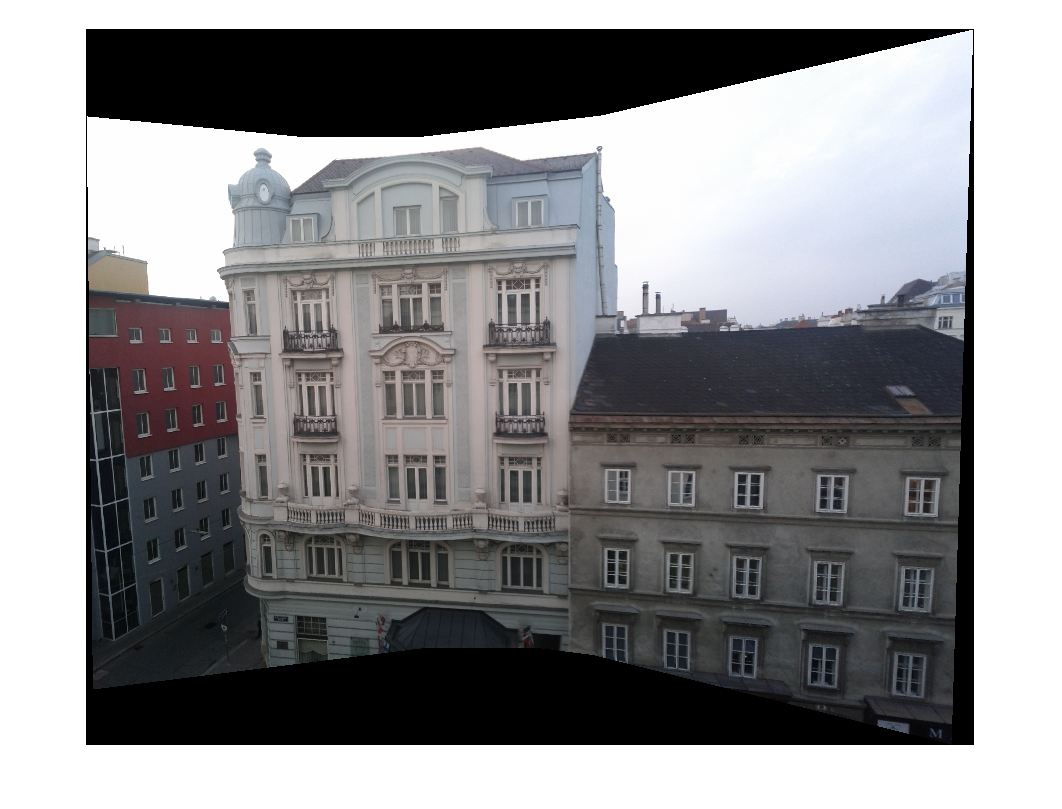
\includegraphics[width=0.8\textwidth]{figures/office_p.png} \\
	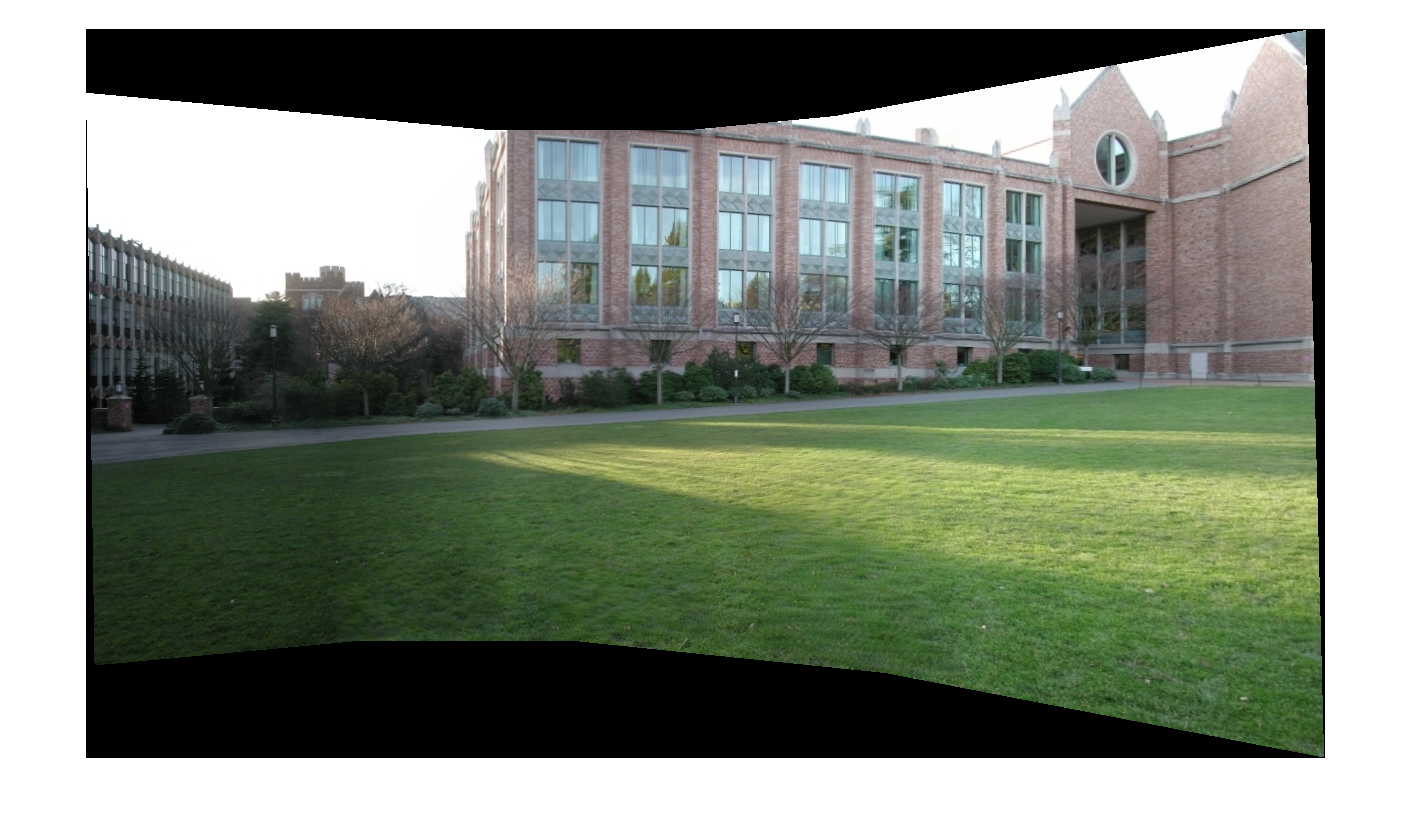
\includegraphics[width=0.8\textwidth]{figures/campus_p.png} 

	\end{tabular}
	\caption{Resulting panorama images with feathering.}
	\label{fig:a4:pano1}
\end{figure}

\begin{figure}[h]
	\centering
	\begin{tabular}{cc}
	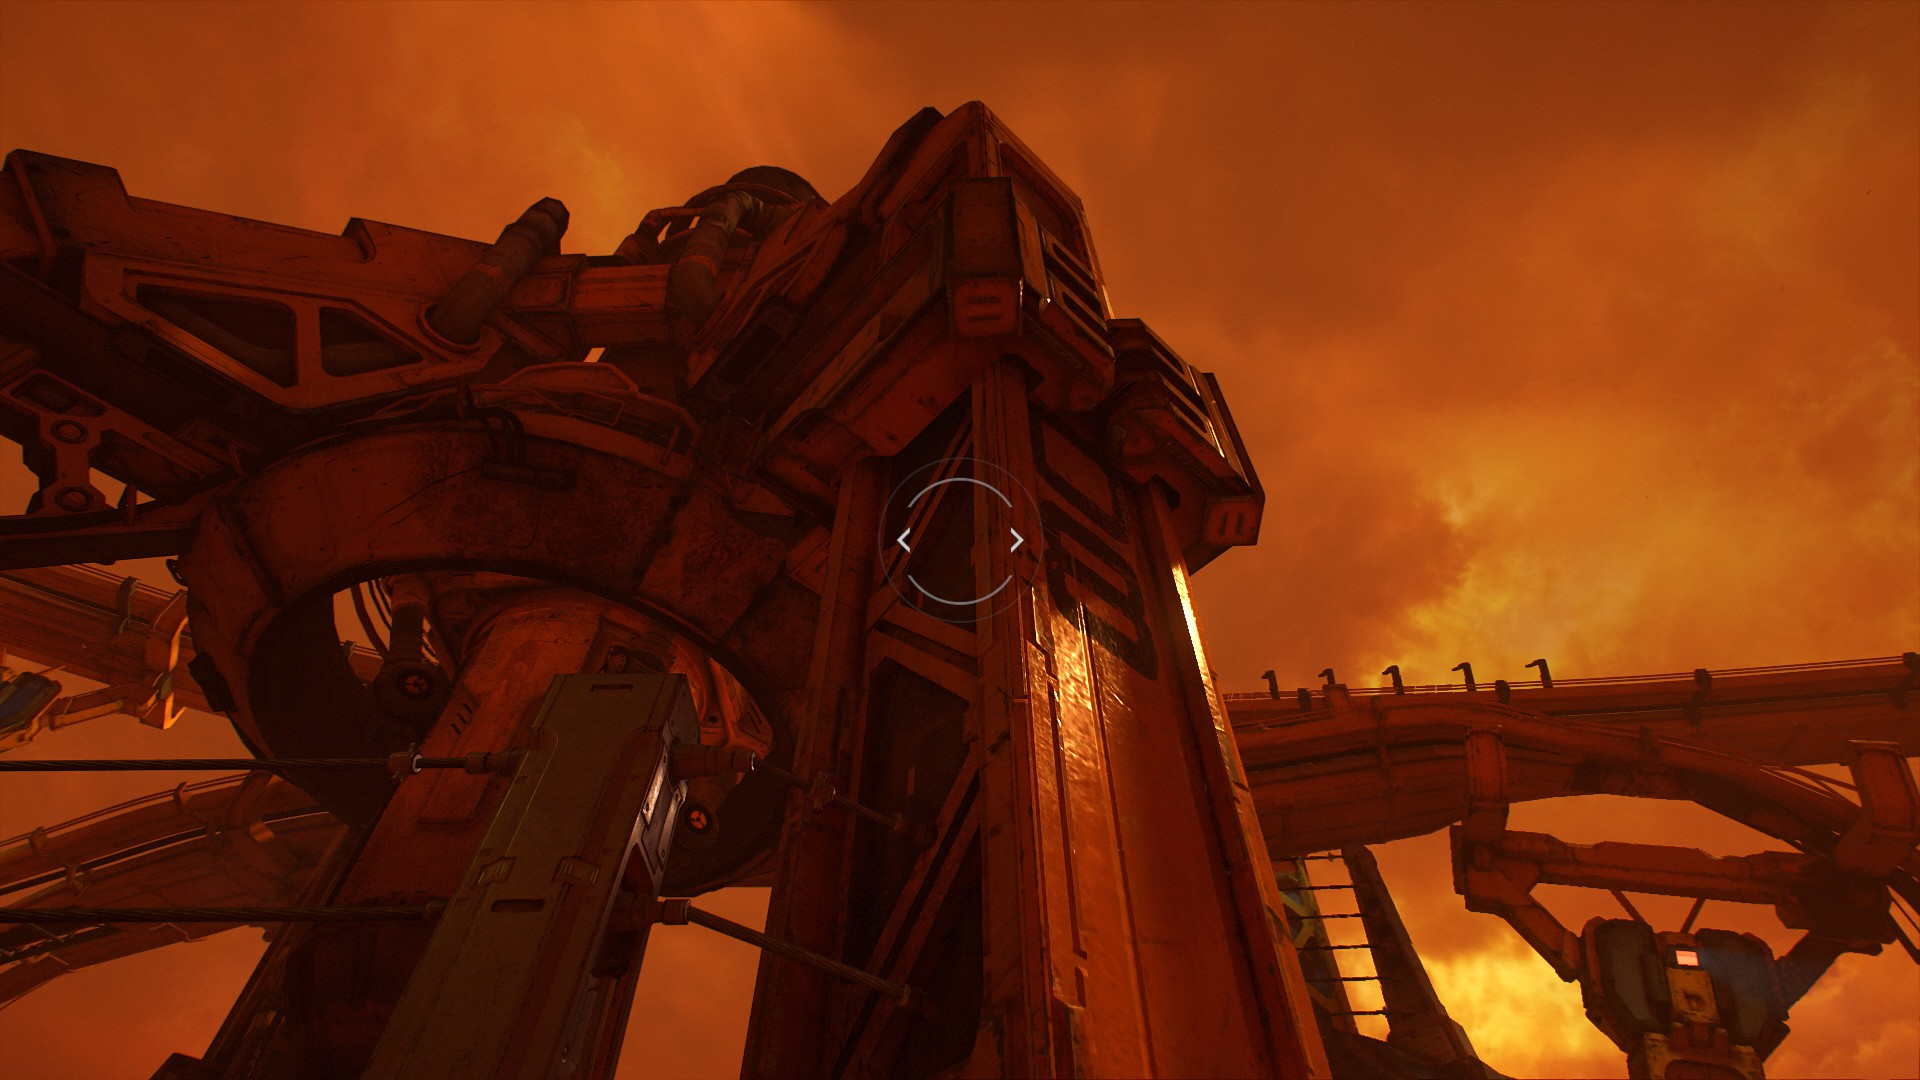
\includegraphics[width=0.33\textwidth]{figures/doom1.jpg}
	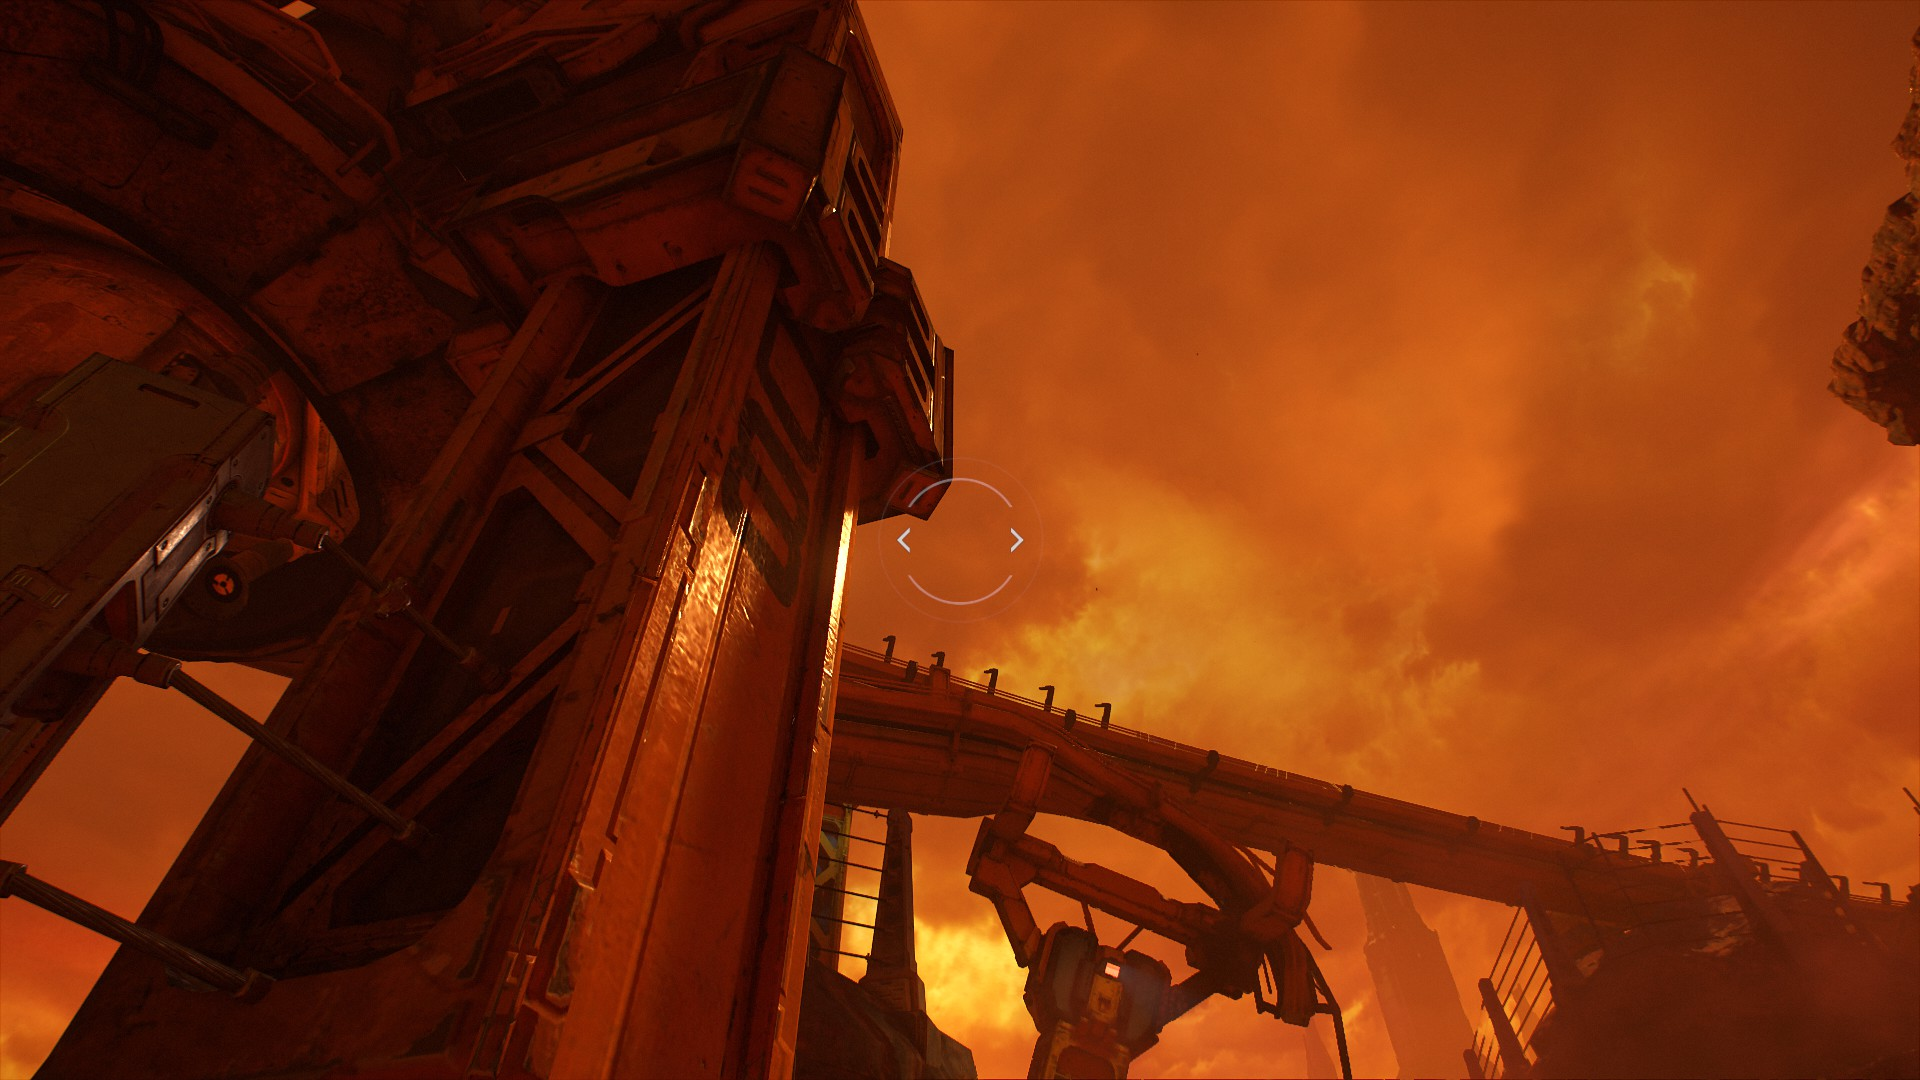
\includegraphics[width=0.33\textwidth]{figures/doom2.jpg}
	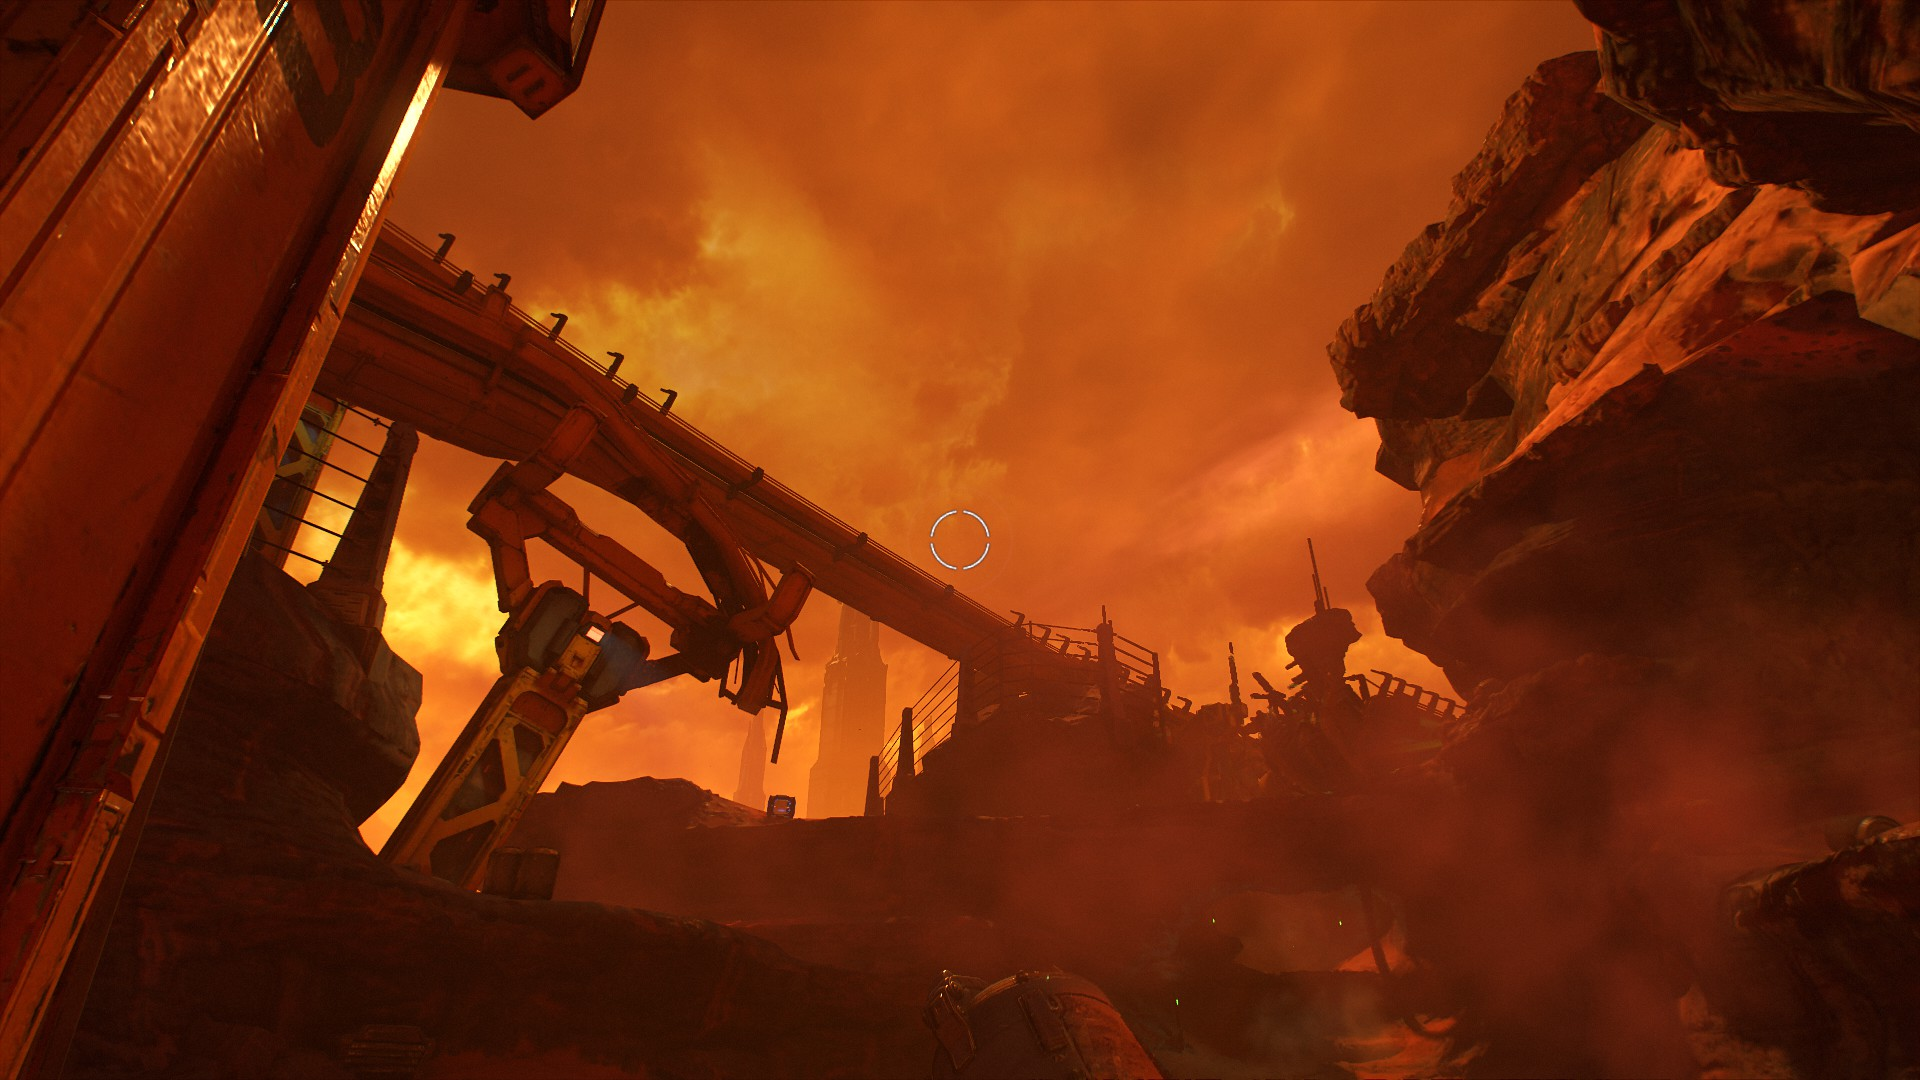
\includegraphics[width=0.33\textwidth]{figures/doom3.jpg} \\
	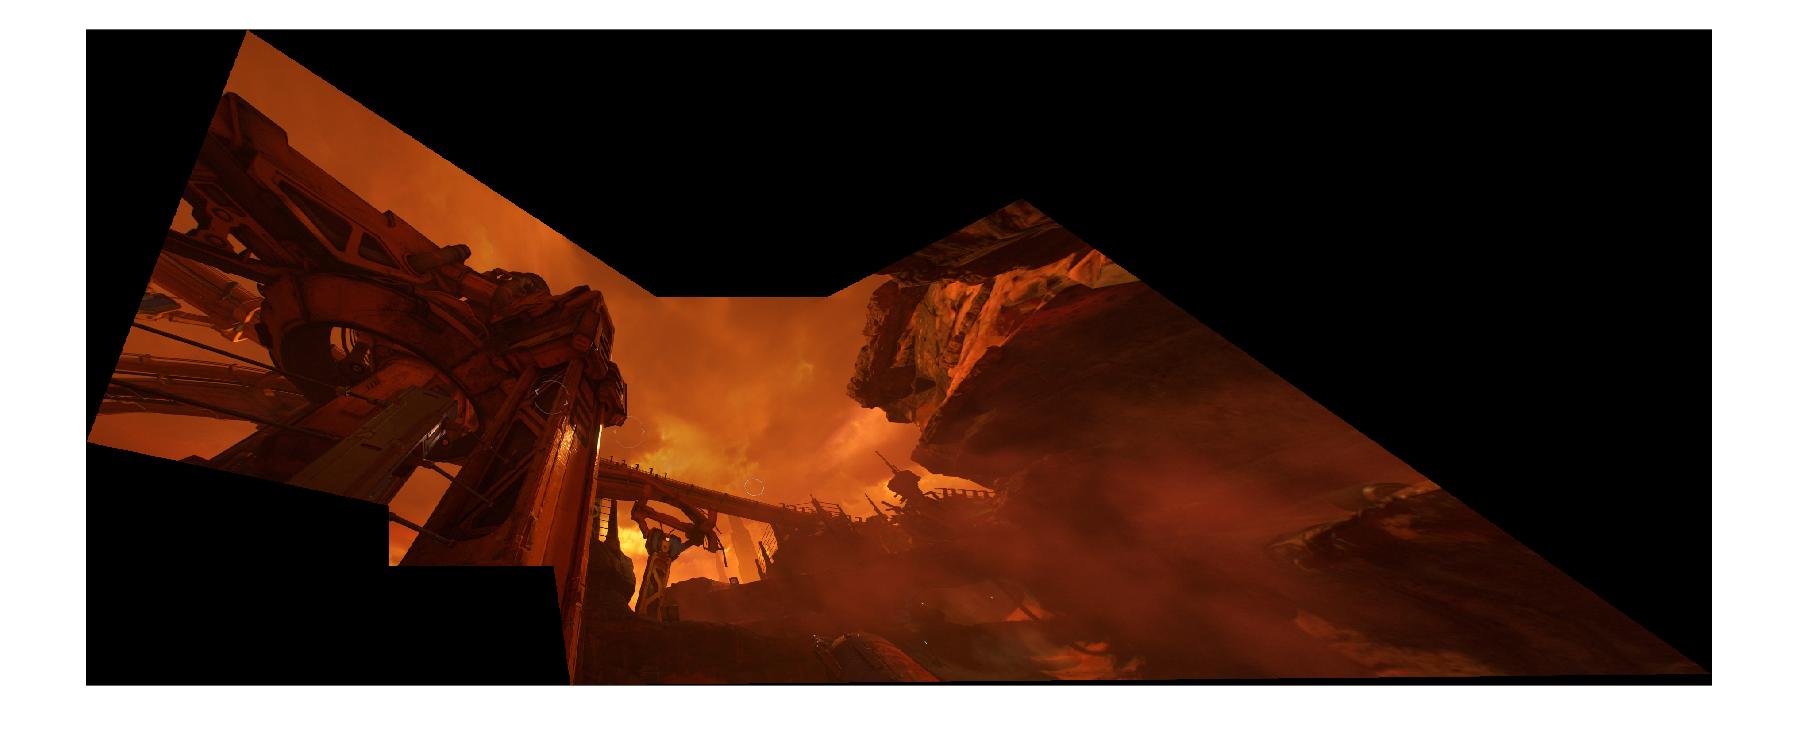
\includegraphics[width=1\textwidth]{figures/doom_p.png}
	
	\end{tabular}
	\caption{Screenshots from the game DOOM (feathering).}
	\label{fig:a4:pano2}
\end{figure}

//note: find and add potential errors here

The panorama images shown in figures \ref{fig:a4:pano1} and \ref{fig:a4:pano2} use feathering to blend the images together. Would we use no blending, the final panorama image would look quite different as illustrated by Figure \ref{fig:a4:noblend}.

\begin{figure}[h]
	\centering
	\begin{tabular}{cc}
	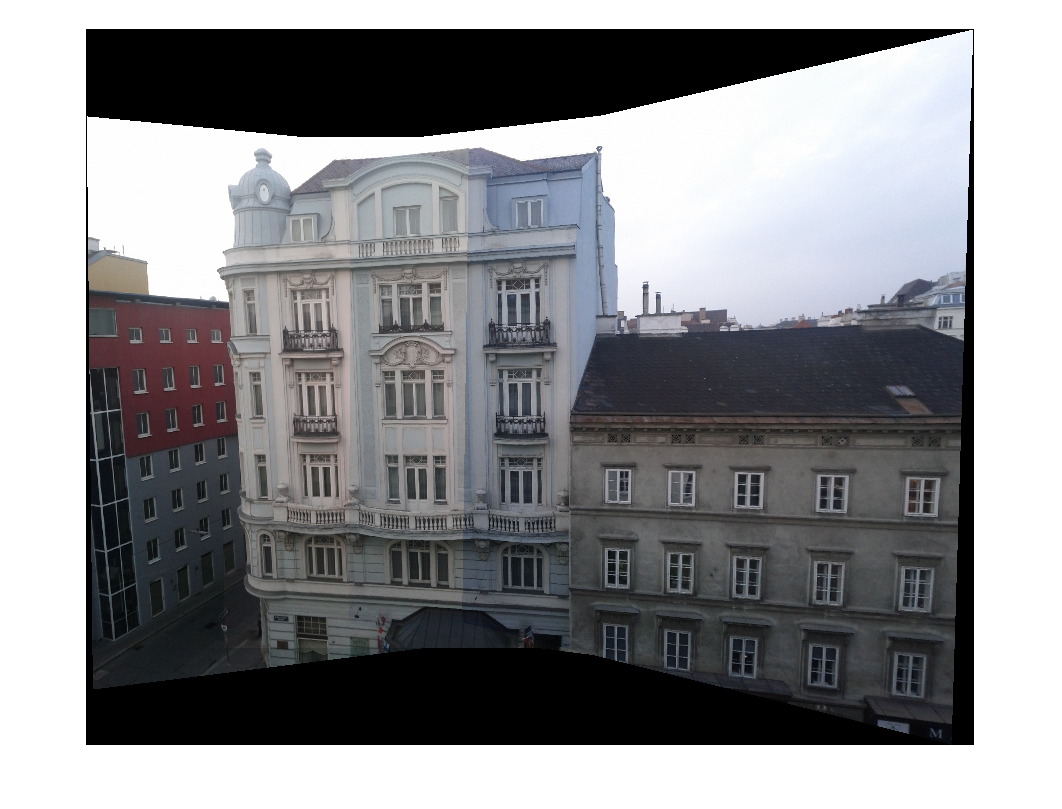
\includegraphics[width=0.8\textwidth]{figures/office_p_b.png} \\
	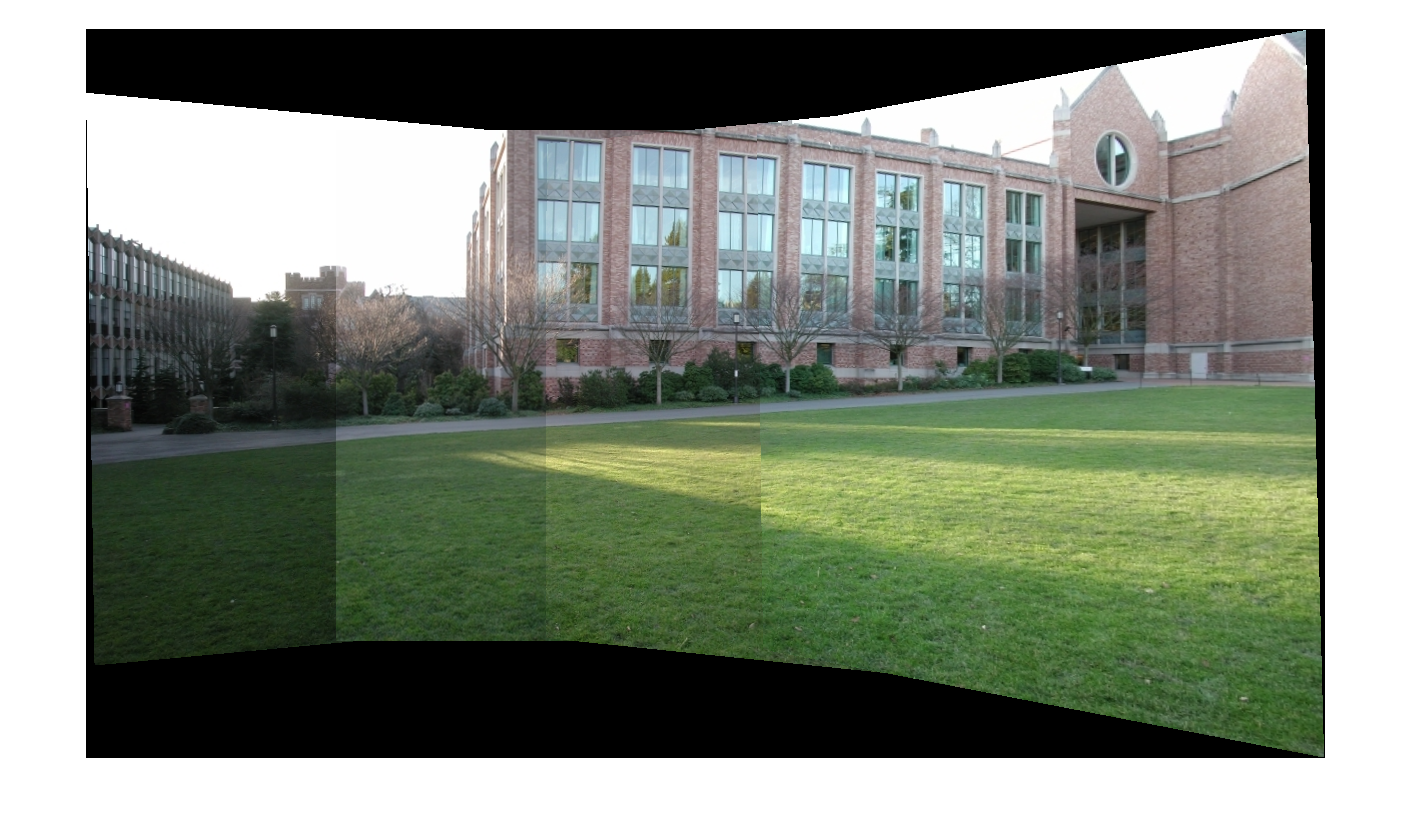
\includegraphics[width=0.8\textwidth]{figures/campus_p_b.png} \\
	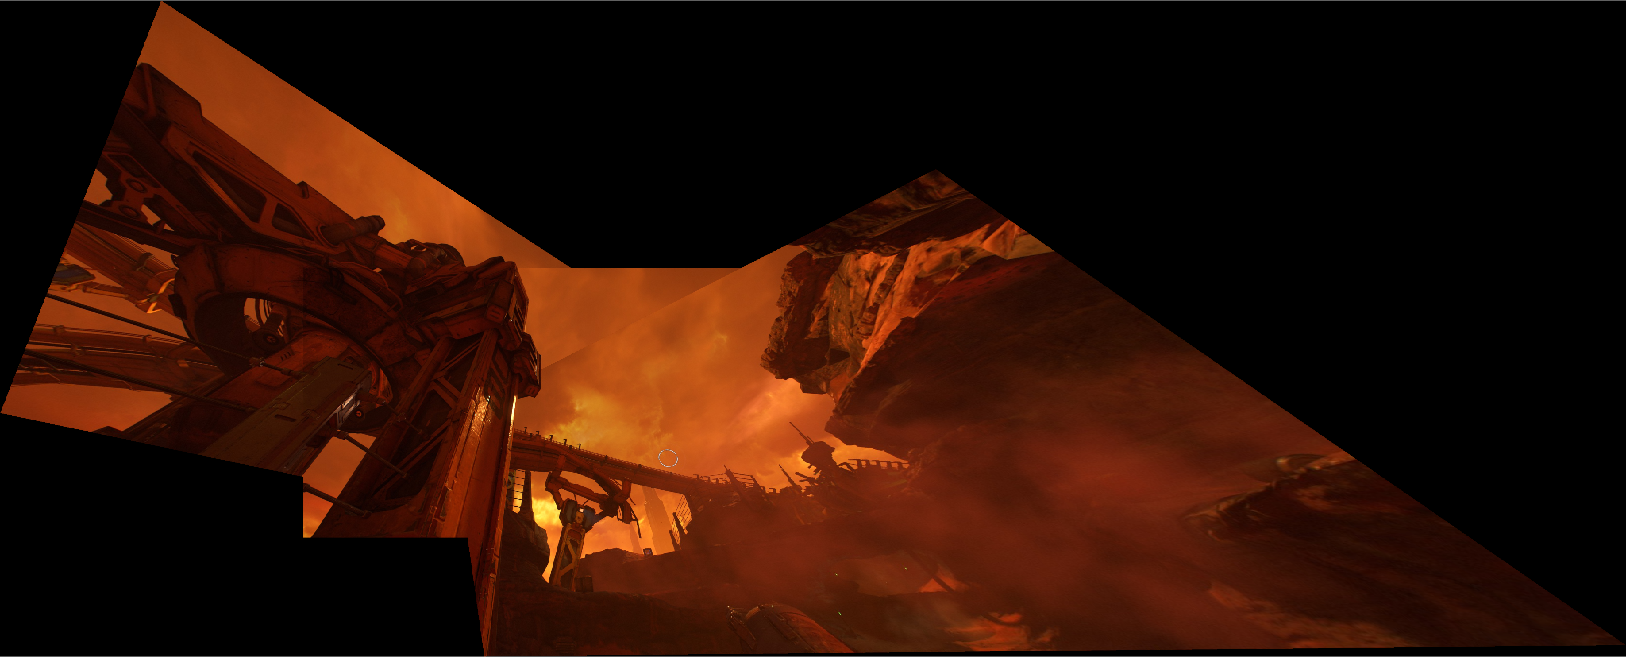
\includegraphics[width=1\textwidth]{figures/doom_p_b.png}

	\end{tabular}
	\caption{Resulting panorama images without blending.}
	\label{fig:a4:noblend}
\end{figure}
\FloatBarrier % keep figures above!

\section{Assignment 5: Scene Recognition with Bag of Visual Words}

The goal of this section is to map any test image to 8 pre-defined scenes described by a training set of images. For this purpose, we try to create a vocabulary of visual words. The goal of a visual word is to be the most expressive descriptor for a type of interest point. As the first step, we use \texttt{vl\_dsift} to get around 100 descriptors from each image on the training collection. We perform k-means clustering on the list of all resulting descriptors to get our visual words. Each visual word therefore is the centroid of a cluster of 128 numbers long SIFT descriptors.


In our tests we utilized both 50 and 75 clusters/visual words.


Once the vocabulary is complete, we need to create a map between the existing training images and our visual words. First we use \texttt{vl\_dsift} to extract the key points of each training image, however this time with a smaller step size. For the exact step size 2 was chosen as the results did not improve with the size of 1. Next we use knnsearch to find the nearest visual word in vocabulary for each SIFT descriptor of the image. Finally we create a (normalized) histogram for each image representing the occurrence count of each visual word in the image. The collection of all histograms(training) and the associated image classes (group) is returned by the function \texttt{BuildKNN}.


The next step is to test images against our model as an attempt to recognize the scene correctly. Again, we use \texttt{vl\_dsift} and create a histogram as described above. As the function \texttt{knnclassify} is removed in MATLAB2018 we used the combination of functions \texttt{fitcknn} and \texttt{predict} to guess the correct scene. The result of the prediction compared to the actual class of the image is reflected by the confusion matrix.

Figures \ref{fig:a5:50c3nn2s} to \ref{fig:a5:75c21nn2s} visualize the precision rate and the confusion matrix for different sizes of vocabulary, step parameter and number of neighbors.


\begin{figure}[h]
	\centering
	\begin{subfigure}{0.3\textwidth}
		\begin{subfigure}[t]{\textwidth}
			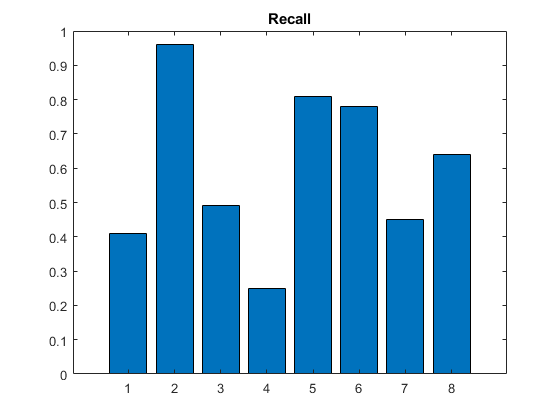
\includegraphics[width=\textwidth]{figures/recall_50C_3NN_2S.png} 
			\caption{Recall}
		\end{subfigure}
		\begin{subfigure}[t]{\textwidth}
			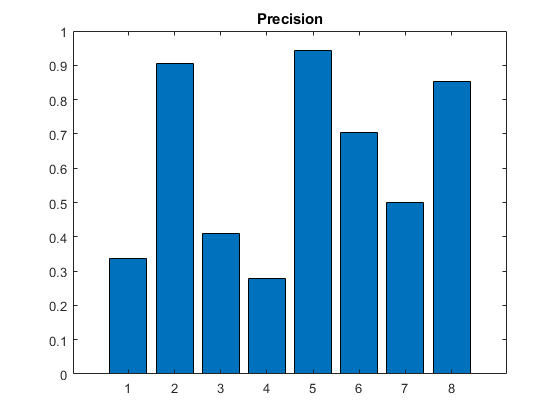
\includegraphics[width=\textwidth]{figures/precision_50C_3NN_2S.png}
			\caption{Precision}
		\end{subfigure}

	\end{subfigure}
	\begin{subfigure}{0.65\textwidth}
		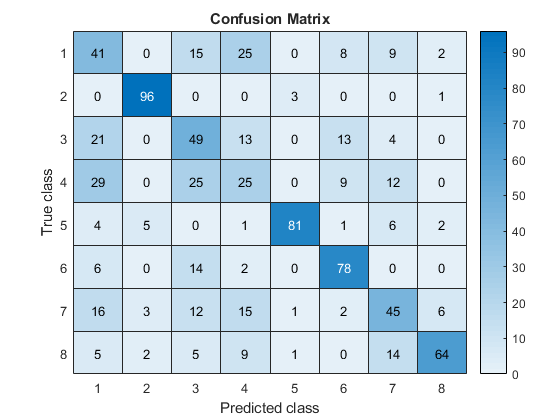
\includegraphics[width=\textwidth]{figures/confusion_50C_3NN_2S.png}
		\caption{Confusion Matrix}
	\end{subfigure}
	\caption{Results for numClusters = 50, numNeighbors = 3 and step size of 2. Success rate is 59.9\%.}
	\label{fig:a5:50c3nn2s}
\end{figure}

\begin{figure}[h]
	\centering
	\begin{subfigure}{0.3\textwidth}
		\begin{subfigure}[t]{\textwidth}
			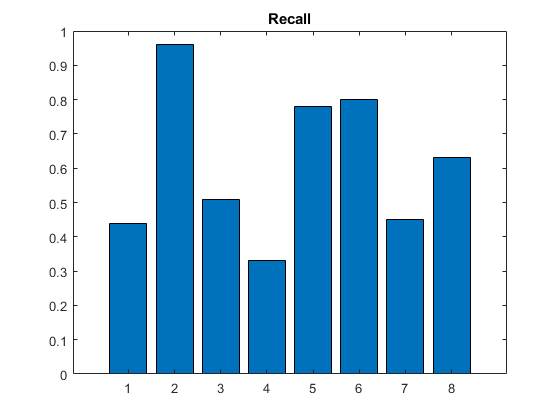
\includegraphics[width=\textwidth]{figures/recall_75C_3NN_2S.png} 
			\caption{Recall}
		\end{subfigure}
		\begin{subfigure}[t]{\textwidth}
			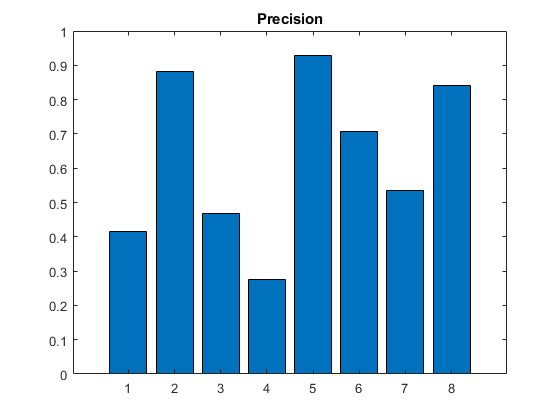
\includegraphics[width=\textwidth]{figures/precision_75C_3NN_2S.png}
			\caption{Precision}
		\end{subfigure}

	\end{subfigure}
	\begin{subfigure}{0.65\textwidth}
		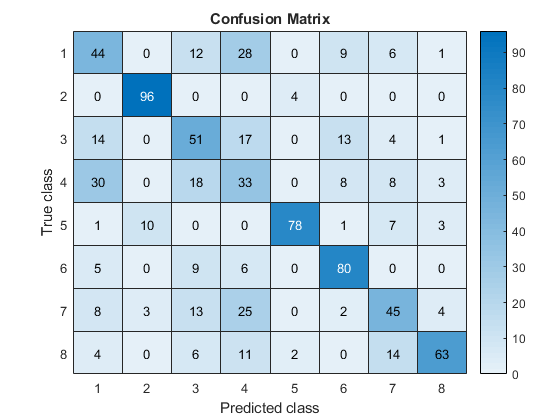
\includegraphics[width=\textwidth]{figures/confusion_75C_3NN_2S.png}
		\caption{Confusion Matrix}
	\end{subfigure}
	\centering
	\caption{Results for numClusters = 75, numNeighbors = 3 and step size of 2. Success rate is 61.3\%.}
	\label{fig:a5:75c3nn2s}
\end{figure}

\begin{figure}[h]

	\centering
	\begin{subfigure}{0.3\textwidth}
		\begin{subfigure}[t]{\textwidth}
			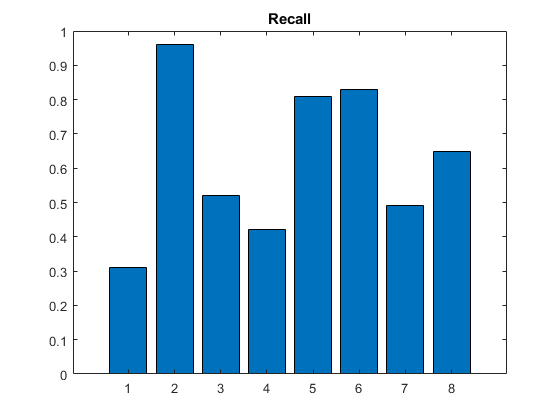
\includegraphics[width=\textwidth]{figures/recall_75C_5NN_2S.png} 
			\caption{Recall}
		\end{subfigure}
		\begin{subfigure}[t]{\textwidth}
			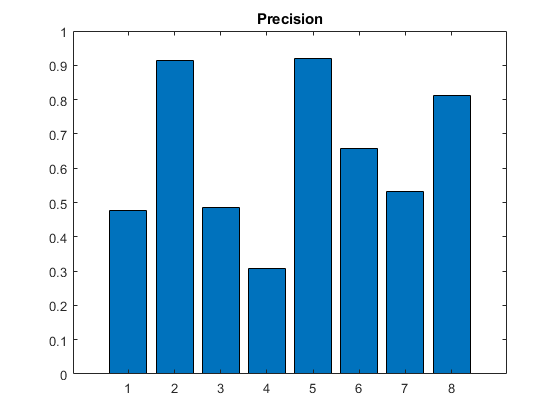
\includegraphics[width=\textwidth]{figures/precision_75C_5NN_2S.png}
			\caption{Precision}
		\end{subfigure}

	\end{subfigure}
	\begin{subfigure}{0.65\textwidth}
		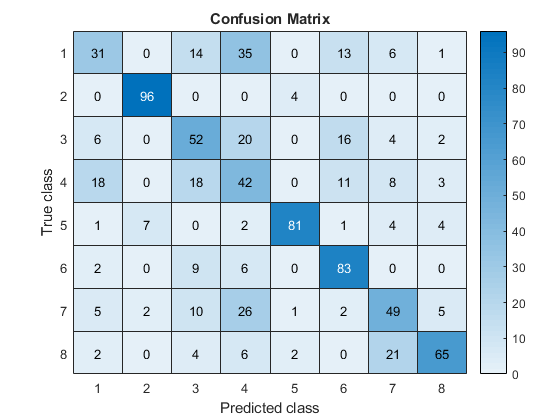
\includegraphics[width=\textwidth]{figures/confusion_75C_5NN_2S.png}
		\caption{Confusion Matrix}
	\end{subfigure}
	\caption{Results for numClusters = 75, numNeighbors = 5 and step size of 2. Success rate is 62.4\%.}
	\label{fig:a5:75c5nn2s}
\end{figure}

\begin{figure}[h]
	\centering
	\begin{subfigure}{0.3\textwidth}
		\begin{subfigure}[t]{\textwidth}
			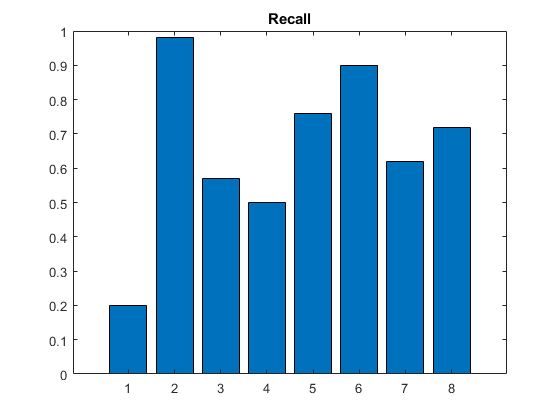
\includegraphics[width=\textwidth]{figures/recall_75C_21NN_2S.png} 
			\caption{Recall}
		\end{subfigure}
		\begin{subfigure}[t]{\textwidth}
			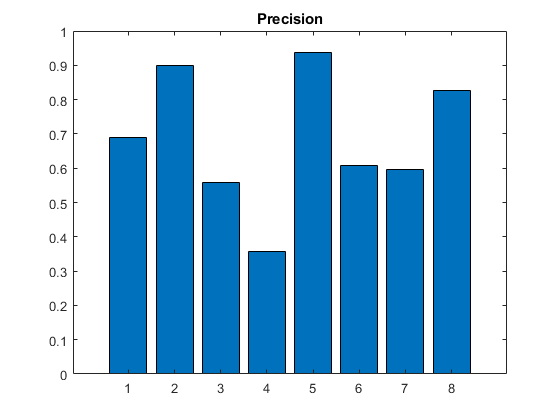
\includegraphics[width=\textwidth]{figures/precision_75C_21NN_2S.png}
			\caption{Precision}
		\end{subfigure}

	\end{subfigure}
	\begin{subfigure}{0.65\textwidth}
		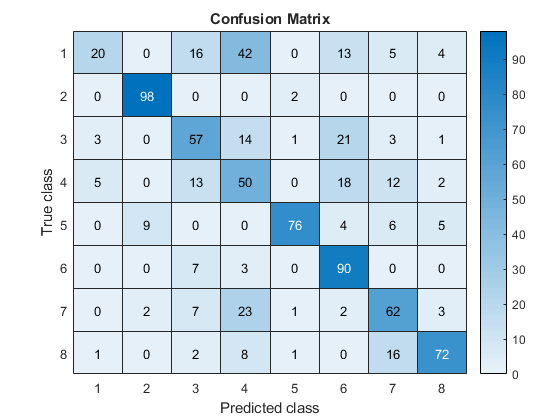
\includegraphics[width=\textwidth]{figures/confusion_75C_21NN_2S.png}
		\caption{Confusion Matrix}
	\end{subfigure}

	\caption{Results for numClusters = 75, numNeighbors = 21 and step size of 2. Success rate is 65.6\%.}
	\label{fig:a5:75c21nn2s}
\end{figure}

As illustrated by the diagrams, the success rates of the classes mountain, forest and street is quite high. The classes bedroom, kitchen and living room have a high rate of confusion with each other. Especially the living room's bad detection rate is mostly due to the other 2 categories. There is a certain confusion between mountain and forest, however that can be seen as expected.

// self test images
\FloatBarrier % keep figures above!


\end{document}

%%% Local Variables: 
%%% mode: latex
%%% TeX-master: t
%%% End: 

